\clearpage
\section{Multirobot problem}
\subsection{Problem definition and states}

The different between single robot problem and multi robot problem is, every robot take turns to make actions, and it needs collision detection. In thiscase, we decide the a whole state for all the $k$ robots, like this:



$$\begin{pmatrix}
x_0 & y_0 \\
x_1 & y_1 \\
\vdots & \vdots \\	
x_{k-1} & y_{k-1}
\end{pmatrix}$$
However, this is not enough for the states. We still one parameter, which the turn of the robot. This parameter is not necessary, which means you can still solve the problem without it in the state. However, returning all the possible states of $k$ can be very redundant and time consumming for latter searching. If I have k robot, and five actions (4 directions plus not moving), the upper bound of states would be $5^k$. It is like giving too much options more next step, while I am not making any decision.











\subsection{Discussions}
ith $n\times n$ size of maze and $k$ robots, the upper bound of this problem, meaning to neglect the legal problem, is $n^k$. Because each robot has $n$ possible position.

If number of wall square is $w$, then the number of collisions would be total state minus legal states, $(n-w)^k - C_{n-w}^k$.

As for $100\times100$, with a few walls and several robot discussion. States number grows exponentially with $k$, and bfs tends to search all the state starting from start node. I think this problem still depends on whether the goal is close to the starting point.

As for the design of heuristic, I will use the following function,
$h = \sum^{k-1}_{i=0}h_i$, where $h_i$ represents the Manhattan distance from robot $i$ to the goal. A function is monotonic as long as\footnote{from \url{wiki: http://en.wikipedia.org/wiki/Consistent_heuristic}}:

$$h(N) \leq c(N,P)+h(P) $$
$$h(G)=0$$
where

\begin{itemize}
\item h is the consistent heuristic function,
\item N is any node in the graph,
\item P is any descendant of N,
\item G is any goal node,
\item c(N,P) is the cost of reaching node P from N.
\end{itemize}

It is obvious that for single robot, the single heuristic satisfy this condtions. An extreme case is the empty maze, where $h(N) = c(N,P)+h(P) $. In any other kind of maze, due to the obstacles, the $h$ usually larger than $cost$, because Manhattan distance is the shortest distance.

Under the condition that single heuristic satisfy this condtions. Adding them together should not affect the monotonicity.

The 8-puzzle problem is the case of multi-robot where there is no walls, and there is only one free space to move, and the goal is letting each robots move to its corresponding positions.

Whether 8-puzzle can be divided into two disjoint? This is similar to graph connectivity problem, or disjoint set problem. There is no better way but to traverse through all the possible states in 8 puzzle.

Let's say the total I calculate that the total states amount of this problem is $N$. My basic idea is, first I pick an arbitrary state, and use bfs to traverse all the connected states, push every one of them into a \textbf{hash set}. At this point the number of the set should be less then $N$. (Otherwise we turn out to prove there is no disjoint set.) Then I will pick antoher state that is not blong to the first set, and also use bfs to create another \textbf{hash set}. Finally, the sum of this two set should equal to $N$.



















\subsection{Code implementation}


\subsubsection{getSuccessors}

\textbf{getSuccessors} is used to expand new states from the current state.

\textbf{Line 4:} Iterate through all the 5 possible actions (4 directions plus not moving).
\textbf{Line 6-7:} Initiate the coordinates for the successor's state, noted that only the robot in turn can take action here.
\textbf{Line 11-13:} Construct the successor with new coordinates, and new cost based on whether it moves, and also keep looping the turn through $R$ robots.

\begin{lstlisting}[numbers=left]
public ArrayList<SearchNode> getSuccessors() {
  ArrayList<SearchNode> successors = new ArrayList<SearchNode>();
  Integer[] xNew = new Integer[R], yNew = new Integer[R];
  // take actions
  for (int[] action : actions) {
    for (int r = 0; r < R; r++) {
      xNew[r] = robots[r][0] + action[0] * (r == turn ? 1 : 0);
      yNew[r] = robots[r][1] + action[1] * (r == turn ? 1 : 0);
    }
    if (maze.isLegal(xNew[turn], yNew[turn])
        && noCollision(xNew, yNew)) {
      SearchNode succ = new MultirobotNode(xNew, yNew, getCost()
          + Math.abs(action[0]) + Math.abs(action[1]),
          (turn + 1) % R);
      successors.add(succ);
    }
  }
  return successors;
}
\end{lstlisting}


\subsubsection{noCollision}

\textbf{noCollision} is used to determine whether there is a collision of robots. I set it as private seems it is not used for outter class.

The basic idea is, I hash the position of each robot, and and check if the hash code already exists. If so, means there is another robot at this coordinate $(x,y)$; if not, push it into the hash set.

If I implement \textbf{noCollision} in simple iteration, the time complexity would be $O(k^2)$, while $k$ is the number of robots. By doing so, I reduce time complexity to $O(k)$.

\begin{lstlisting}[numbers=left]
private boolean noCollision(Integer[] xNew, Integer[] yNew) {
  HashSet<Integer> existed = new HashSet<>();
  for (int r = 0; r < R; r++) {
    Integer tmpHash = oneHash(xNew[r], yNew[r]);
    if (!existed.contains(tmpHash)) {
      existed.add(tmpHash);
    } else {
      return false;
    }
  }
  return true;
}
\end{lstlisting}




\subsubsection{Ohter methods}
Node constructor, it initiates the positions of robots iteratively.

\begin{lstlisting}[numbers=left]
public MultirobotNode(Integer[] x, Integer[] y, double c, int t) {
  robots = new int[R][2];
  for (int i = 0; i < R; i++) {
    this.robots[i][0] = x[i];
    this.robots[i][1] = y[i];
  }
  turn = t;
  cost = c;
}
\end{lstlisting}

Change the heuristic method to interative way.

\begin{lstlisting}[numbers=left]
public double heuristic() {
  // manhattan distance metric for simple maze with one agent:
  double hValue = 0;
  for (int i = 0; i < R; i++)
    hValue += Math.abs(xGoal[i] - robots[i][0])
        + Math.abs(yGoal[i] - robots[i][1]);
  return hValue;
}
\end{lstlisting}

\textbf{Line 20-28:} After poping the node, we check for two condition. One is if it is the goal, we simply return the solution path and terminate the search. Antoher condition is, if the node has been visited before, we don't push it into \emph{frontiers} unless it has shorter cost than before.

\textbf{Line 29-35:} Get the successors of currrent node, and push those un-visited nodes or node has shorter cost than before, into the \emph{frontiers}.



\subsection{Output demonstration}

Output of shifting 3 robots If we substract start and end, we know averagely every robot take 4 actions, that is acceptable in a wall-free space. (Figure \ref{m-1}):
\begin{lstlisting}[numbers=left]
A*:
path length: 14
Nodes explored during search: 167
Maximum space usage during search 577
\end{lstlisting}

Output of reodering robot in narrow corridor The path length is much longer that I expected. I guess it is because for an amount of time the robot just stay still, waiting for others. It is not easy to move in a narrow space. (Figure \ref{m-2}):
\begin{lstlisting}[numbers=left]
A*:
path length: 52
Nodes explored during search: 953
Maximum space usage during search 861
\end{lstlisting}


Output of cross road conflict. The average number of movements is 9, which is also reasonable. (Figure \ref{m-3}):
\begin{lstlisting}[numbers=left]
A*:
path length: 20
Nodes explored during search: 105
Maximum space usage during search 177
\end{lstlisting}

Output of moving relatively large number of robots. (Figure \ref{m-4}):
\begin{lstlisting}[numbers=left]
A*:
path length: 115
Nodes explored during search: 5070107
Maximum space usage during search 9081343
\end{lstlisting}

Output of moving relatively large maze. Noted that, although path length is much longer than the previous one, the explored nodes is actually much less. This is because states space size grow expoentially with number of robots. (Figure \ref{m-5}):
\begin{lstlisting}[numbers=left]
path length: 233
Nodes explored during search: 109132
Maximum space usage during search 184020
\end{lstlisting}


\begin{figure*}[!t]
% ensure that we have normalsize text
\normalsize
% Store the current equation number.
% Set the equation number to one less than the one
% desired for the first equation here.
% The value here will have to changed if equations
% are added or removed prior to the place these
% equations are referenced in the main text.
\centering
\subfigure[start]{
\label{m-1-3} %% label for first subfigure
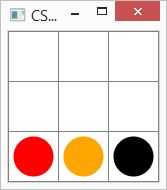
\includegraphics[width=0.16\textwidth]{m-1-3.JPG}}
\subfigure[step 1]{
\label{m-1-0} %% label for second subfigure
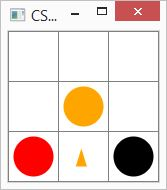
\includegraphics[width=0.16\textwidth]{m-1-0.JPG}}
\subfigure[step 2]{
\label{m-1-1} %% label for second subfigure
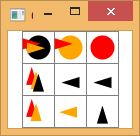
\includegraphics[width=0.16\textwidth]{m-1-1.JPG}}
\subfigure[step 3]{
\label{m-1-2} %% label for second subfigure
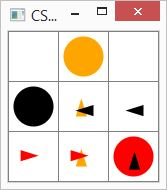
\includegraphics[width=0.16\textwidth]{m-1-2.JPG}}
\subfigure[end]{
\label{m-1-4} %% label for second subfigure
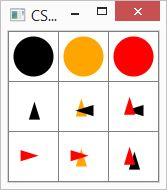
\includegraphics[width=0.16\textwidth]{m-1-4.JPG}}
\caption{Demo of shifting 3 robots}
\label{m-1} %% label for entire figure
\end{figure*}

\begin{figure*}[!t]
% ensure that we have normalsize text
\normalsize
% Store the current equation number.
% Set the equation number to one less than the one
% desired for the first equation here.
% The value here will have to changed if equations
% are added or removed prior to the place these
% equations are referenced in the main text.
\centering
\subfigure[start]{
\label{m-2-0} %% label for first subfigure
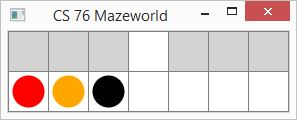
\includegraphics[width=0.206\textwidth]{m-2-0.JPG}}
\subfigure[step 1]{
\label{m-2-0} %% label for first subfigure
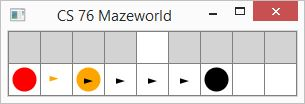
\includegraphics[width=0.206\textwidth]{m-2-1.JPG}}
\subfigure[step 2]{
\label{m-2-0} %% label for first subfigure
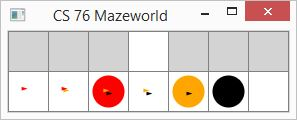
\includegraphics[width=0.206\textwidth]{m-2-2.JPG}}
\subfigure[step 3]{
\label{m-2-0} %% label for first subfigure
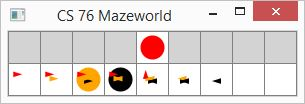
\includegraphics[width=0.206\textwidth]{m-2-3.JPG}}
\subfigure[step 4]{
\label{m-2-0} %% label for first subfigure
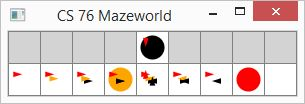
\includegraphics[width=0.206\textwidth]{m-2-4.JPG}}
\subfigure[step 5]{
\label{m-2-0} %% label for first subfigure
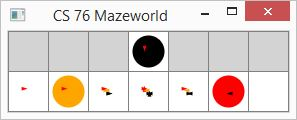
\includegraphics[width=0.206\textwidth]{m-2-5.JPG}}
\subfigure[step 6]{
\label{m-2-0} %% label for first subfigure
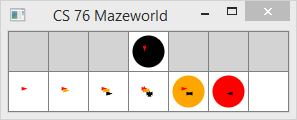
\includegraphics[width=0.206\textwidth]{m-2-6.JPG}}
\subfigure[end]{
\label{m-2-0} %% label for first subfigure
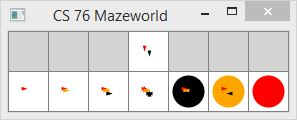
\includegraphics[width=0.206\textwidth]{m-2-7.JPG}}
\caption{Demo of reodering robot in narrow corridor}
\label{m-2} %% label for entire figure
\end{figure*}

\begin{figure*}[!t]
% ensure that we have normalsize text
\normalsize
% Store the current equation number.
% Set the equation number to one less than the one
% desired for the first equation here.
% The value here will have to changed if equations
% are added or removed prior to the place these
% equations are referenced in the main text.
\centering
\subfigure[start]{
\label{m-2-0} %% label for first subfigure
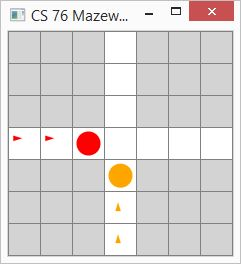
\includegraphics[width=0.206\textwidth]{m-3-0.JPG}}
\subfigure[step 1]{
\label{m-2-0} %% label for first subfigure
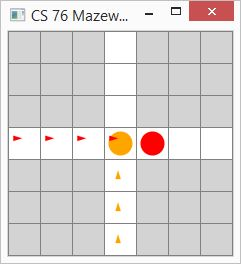
\includegraphics[width=0.206\textwidth]{m-3-1.JPG}}
\subfigure[end]{
\label{m-2-0} %% label for first subfigure
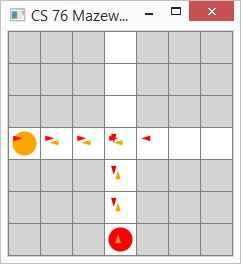
\includegraphics[width=0.206\textwidth]{m-3-2.JPG}}
\caption{Demo of cross road conflict}
\label{m-3} %% label for entire figure
\end{figure*}

\begin{figure*}[!t]
% ensure that we have normalsize text
\normalsize
% Store the current equation number.
% Set the equation number to one less than the one
% desired for the first equation here.
% The value here will have to changed if equations
% are added or removed prior to the place these
% equations are referenced in the main text.
\centering
\subfigure[start]{
\label{m-2-0} %% label for first subfigure
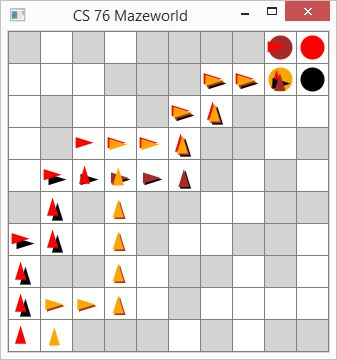
\includegraphics[width=0.618\textwidth]{m-4-1.JPG}}
\caption{Demo of moving relatively large number of robots}
\label{m-4} %% label for entire figure
\end{figure*}

\begin{figure*}[!t]
% ensure that we have normalsize text
\normalsize
% Store the current equation number.
% Set the equation number to one less than the one
% desired for the first equation here.
% The value here will have to changed if equations
% are added or removed prior to the place these
% equations are referenced in the main text.
\centering
\subfigure[start]{
\label{m-2-0} %% label for first subfigure
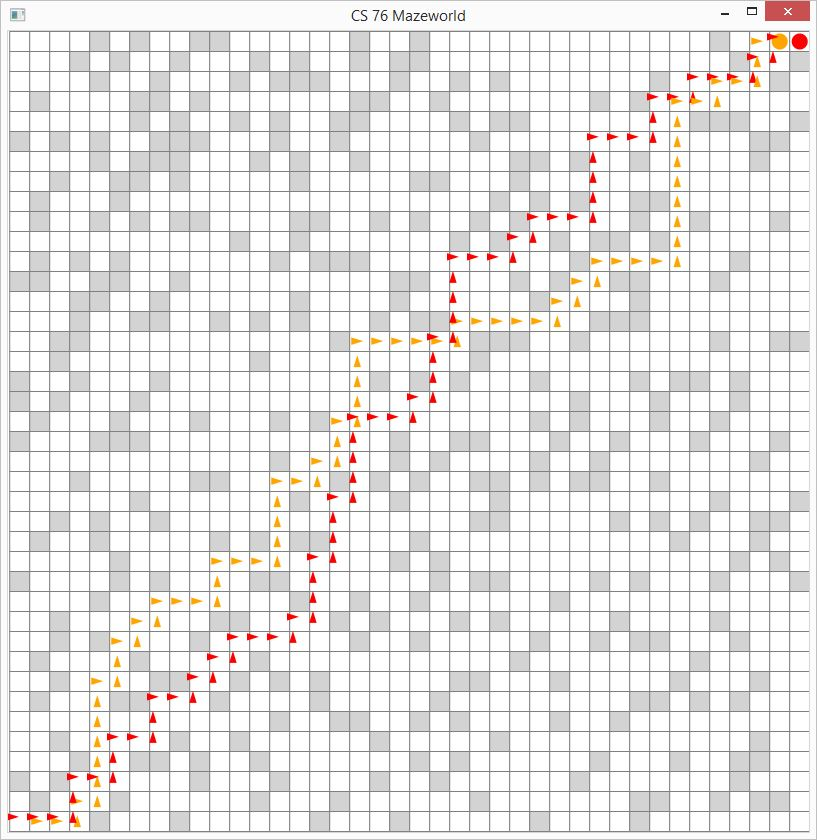
\includegraphics[width=0.818\textwidth]{m-5-1.JPG}}
\caption{Demo of moving relatively large large maze}
\label{m-5} %% label for entire figure
\end{figure*}


